%%%%%%%%%%%%%%%%%%%%%%%%%%%%%%%%%%%%%%%%%
% Beamer Presentation
% LaTeX Template
% Version 1.0 (10/11/12)
%
% This template has been downloaded from:
% http://www.LaTeXTemplates.com
%
% License:
% CC BY-NC-SA 3.0 (http://creativecommons.org/licenses/by-nc-sa/3.0/)
%
%%%%%%%%%%%%%%%%%%%%%%%%%%%%%%%%%%%%%%%%%

%----------------------------------------------------------------------------------------
%	PACKAGES AND THEMES
%----------------------------------------------------------------------------------------

\documentclass{beamer}

\mode<presentation> {

% The Beamer class comes with a number of default slide themes
% which change the colors and layouts of slides. Below this is a list
% of all the themes, uncomment each in turn to see what they look like.

%\usetheme{default}
%\usetheme{AnnArbor}
%\usetheme{Antibes}
%\usetheme{Bergen}
%\usetheme{Berkeley}
%\usetheme{Berlin}
%\usetheme{Boadilla}
%\usetheme{CambridgeUS}
%\usetheme{Copenhagen}
%\usetheme{Darmstadt}
%\usetheme{Dresden}
\usetheme{Frankfurt}
%\usetheme{Goettingen}
%\usetheme{Hannover}
%\usetheme{Ilmenau}
%\usetheme{JuanLesPins}
%\usetheme{Luebeck}
%\usetheme{Madrid}
%\usetheme{Malmoe}
%\usetheme{Marburg}
%\usetheme{Montpellier}
%\usetheme{PaloAlto}
%\usetheme{Pittsburgh}
%\usetheme{Rochester}
%\usetheme{Singapore}
%\usetheme{Szeged}
%\usetheme{Warsaw}

% As well as themes, the Beamer class has a number of color themes
% for any slide theme. Uncomment each of these in turn to see how it
% changes the colors of your current slide theme.

%\usecolortheme{albatross}
%\usecolortheme{beaver}
%\usecolortheme{beetle}
%\usecolortheme{crane}
%\usecolortheme{dolphin}
%\usecolortheme{dove}
%\usecolortheme{fly}
%\usecolortheme{lily}
%\usecolortheme{orchid}
%\usecolortheme{rose}
%\usecolortheme{seagull}
%\usecolortheme{seahorse}
%\usecolortheme{whale}
%\usecolortheme{wolverine}

%\setbeamertemplate{footline} % To remove the footer line in all slides uncomment this line
%\setbeamertemplate{footline}[page number] % To replace the footer line in all slides with a simple slide count uncomment this line

%\setbeamertemplate{navigation symbols}{} % To remove the navigation symbols from the bottom of all slides uncomment this line
}

\usepackage{graphicx} % Allows including images
\usepackage{booktabs} % Allows the use of \toprule, \midrule and \bottomrule in tables
\usepackage[brazilian]{babel}
\usepackage[utf8]{inputenc}
\usepackage[T1]{fontenc}
\usepackage{amsmath}
\usepackage{animate}
\usepackage{amsmath}
\DeclareMathOperator{\atantwo}{atan2}
\newcommand{\angstrom}{\textup{\AA}}

%----------------------------------------------------------------------------------------
%	TITLE PAGE
%----------------------------------------------------------------------------------------

\title[T2]{Trabalho II} % The short title appears at the bottom of every slide, the full title is only on the title page

\author{Bruno Iochins Grisci} % Your name
\institute[UFRGS] % Your institution as it will appear on the bottom of every slide, may be shorthand to save space
{
Universidade Federal do Rio Grande do Sul \\ % Your institution for the title page
\medskip
\textit{bigrisci@inf.ufrgs.br} % Your email address
}
\date{\today} % Date, can be changed to a custom date

\begin{document}

\begin{frame}
\titlepage % Print the title page as the first slide
\end{frame}

\begin{frame}
\frametitle{Sumário} % Table of contents slide, comment this block out to remove it
\tableofcontents % Throughout your presentation, if you choose to use \section{} and \subsection{} commands, these will automatically be printed on this slide as an overview of your presentation
\end{frame}

%----------------------------------------------------------------------------------------
%	PRESENTATION SLIDES
%----------------------------------------------------------------------------------------

%------------------------------------------------
\section{Questão 1} % Sections can be created in order to organize your presentation into discrete blocks, all sections and subsections are automatically printed in the table of contents as an overview of the talk
%------------------------------------------------

\begin{frame}
\frametitle{Implementação}
\begin{itemize}
\item Python;
\item Numpy;
\item Orientado a Objetos;
\item Leitura do PDB: reaproveitada do Trabalho I
\end{itemize}
\end{frame}

\begin{frame}
\frametitle{Formação de ligação peptídica}
\begin{itemize}
\item Leitura dos arquivos .pdb dos aminoácidos;
\item Tratar nomenclatura dos átomos;
\item Átomos N dos aminoácidos são transladados para a origem;
\item Para cada aminoácido:
\begin{itemize}
 \item Remove átomo H;
 \item Move N para posição do átomo OC do aminoácido anterior*;
 \item Salva posição do átomo OC atual;
 \item Remove átomos OC e HOC atuais.
\end{itemize}
\item Primeiro e último aminoácidos são casos especiais;
\item Correção de índices.
\end{itemize}
\footnotesize{
*Posição ajustada para que o comprimento da ligação peptídica seja de $1.32\angstrom$ e correção do ângulo da ligação.
}
\end{frame}

\begin{frame}
\frametitle{Estrutura resultante}
Sequência: VSCEDCPEHCSTQKAQAKCDNDKCVCEPI
\begin{figure}
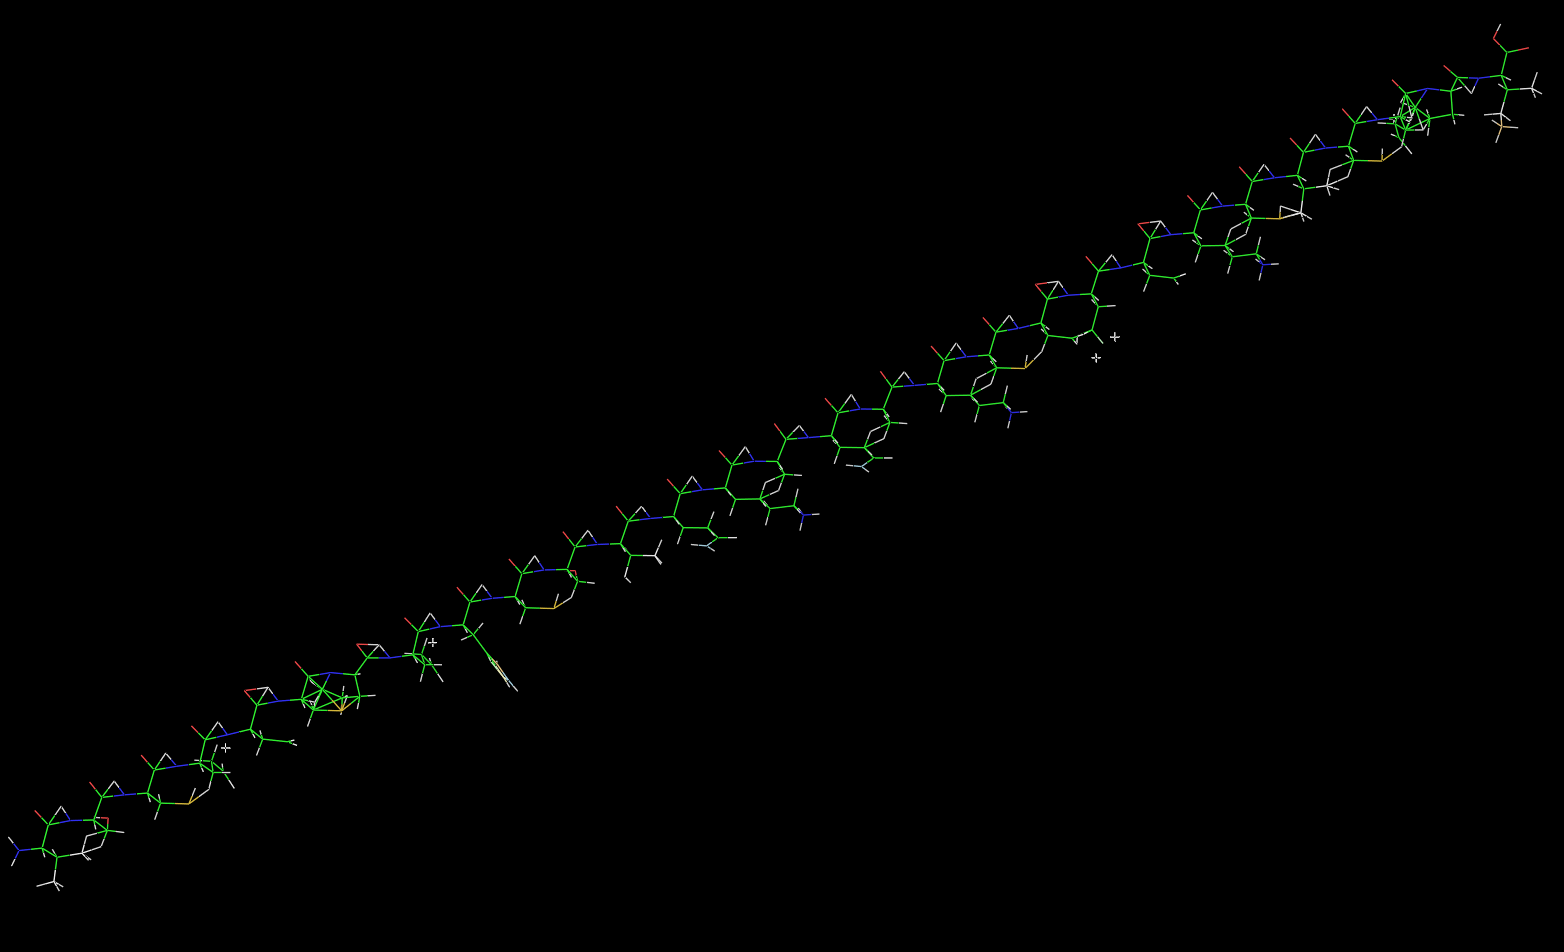
\includegraphics[width=0.8\linewidth]{protein.png}
\end{figure}
\end{frame}

\begin{frame}
\frametitle{Cálculo dos ângulos}
Átomos:
\begin{itemize}
  \item $\phi$ (phi): $C_{n-1} - N_{n} - C_{\alpha n} - C_{n}$
  \item $\psi$ (psi): $N_{n} - C_{\alpha n} - C_{n} - N_{n+1}$
  \item $\omega$ (omega): $C_{\alpha n} - C_{n} - N_{n+1} - C_{\alpha n+1}$
\end{itemize}
\end{frame}

\begin{frame}
\frametitle{Cálculo de ângulo diedro}

\begin{itemize}
 \item $P_{1}, P_{2}, P_{3}, P_{4}$
 \item $\vec{b_{1}} = P_{2} - P_{1}, \vec{b_{2}} = P_{3} - P_{2}, \vec{b_{3}} = P_{4} - P_{3}$
 \item $\vec{n_{1}} = \frac{\vec{b_{1}} \times \vec{b_{2}}}{\parallel \vec{b_{1}} \times \vec{b_{2}} \parallel}$
 \item $\vec{n_{2}} = \frac{\vec{b_{2}} \times \vec{b_{3}}}{\parallel \vec{b_{2}} \times \vec{b_{3}} \parallel}$
 \item $\vec{m_{1}} = \vec{n_{1}} \times \frac{\vec{b_{2}}}{\parallel \vec{b_{2}} \parallel}$
 \item $x = \vec{n_{1}} \cdot \vec{n_{2}}$
 \item $y = \vec{m_{1}} \cdot \vec{n_{2}}$
 \item $\alpha = - \atantwo(y, x)$
\end{itemize}

%n1=\frac{b1\times b2}{\parallel b1\times b2 \parallel}, n2=\frac{b2\times b3}{\parallel b2\times b3 \parallel} \rightarrow m1 = n1\times \frac{b2}{\parallel b2 \parallel}

\end{frame}

\begin{frame}
\frametitle{Ângulos PHI - PSI (1ENY)}
\begin{table}[]
\centering
\label{my-label}
\begin{tabular}{lll}
AMINO ÁCIDO &  PHI     &  PSI    \\
ALA         &  360.00  & -112.08 \\
GLY         &  121.15  &  89.96  \\
LEU         & -52.87   & -30.57  \\
LEU         & -116.76  &  28.04  \\
ASP         & -50.50   &  122.54 \\
GLY         &  62.56   &  31.90  \\
...         & ...      & ...     
\end{tabular}
\end{table}
\end{frame}

\begin{frame}
\frametitle{Ramachandran Map}
\begin{figure}
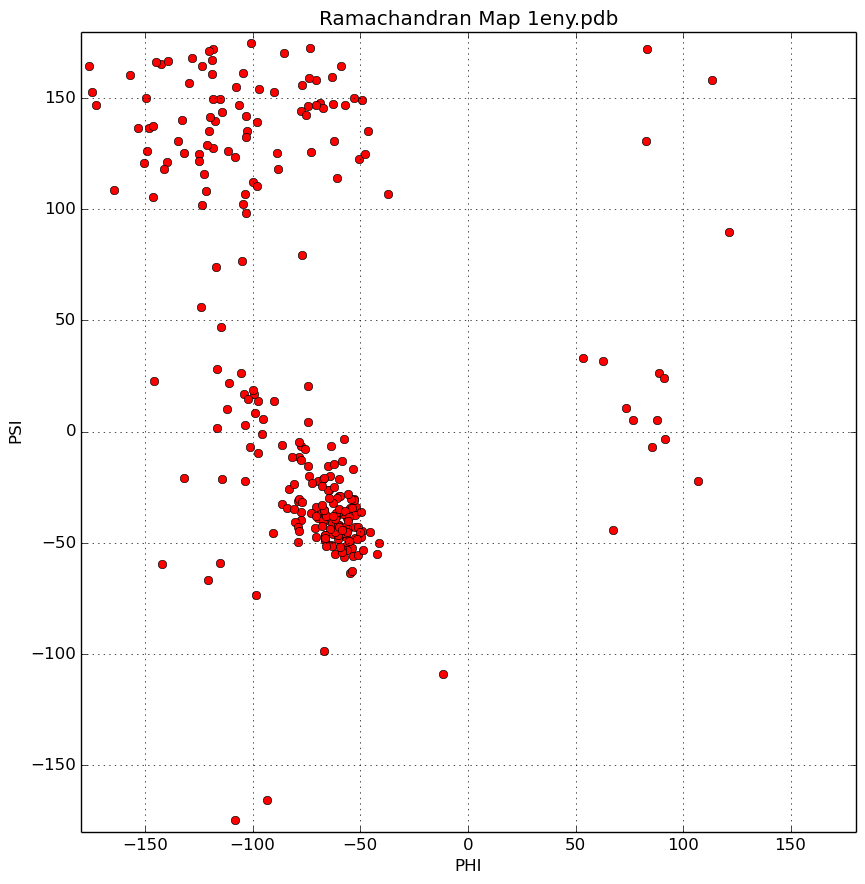
\includegraphics[width=0.6\linewidth]{1eny.png}
\end{figure}
\end{frame}

%------------------------------------------------
\section{Questão 2} 
%------------------------------------------------

\begin{frame}
\frametitle{1PLX-P}
Sequência: YGGFM

$RMSD_{C_\alpha}: 2.931457373$

$RMSD_{backbone}: 2.91612536719$

$RMSD_{all}: 4.75262535547$ 

\begin{figure}
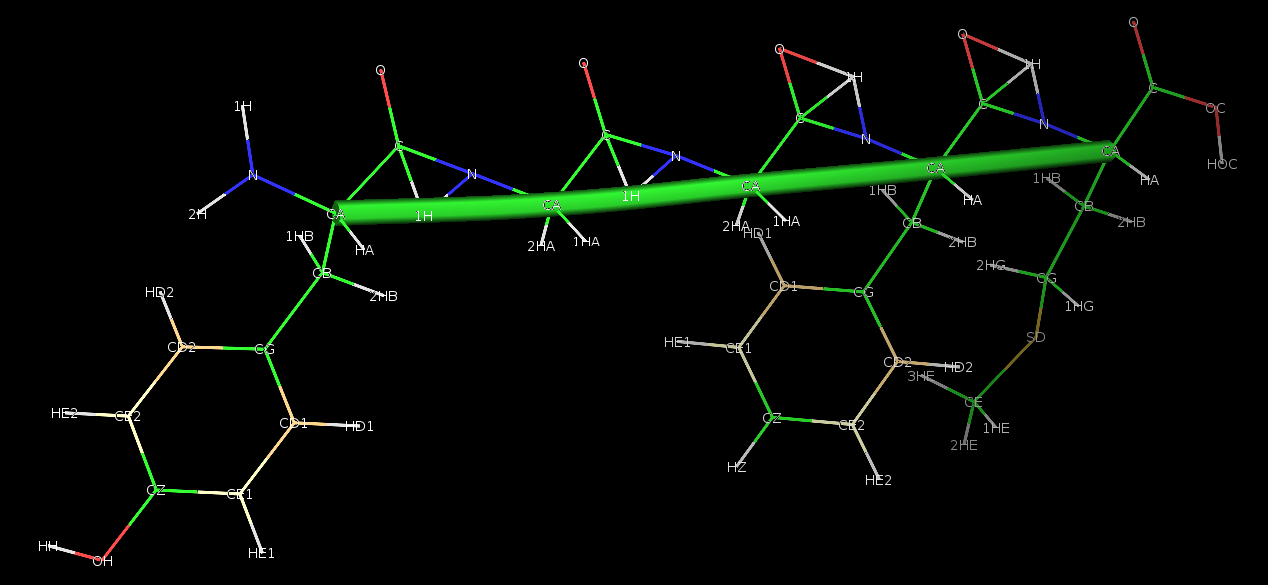
\includegraphics[width=1.0\linewidth]{1PLX-P.png}
\end{figure}
\end{frame}

\begin{frame}
\frametitle{Cálculo do ângulo entre 3 átomos}
\begin{itemize}
 \item $P_{1}, P_{C}, P_{2}$
 \item $\vec{bond_{1C}} = \frac{P_{1} - P_{C}}{\parallel P_{1} - P_{C} \parallel}$
 \item $\vec{bond_{2C}} = \frac{P_{2} - P_{C}}{\parallel P_{2} - P_{C} \parallel}$
 \item $\theta = arccos(\vec{bond_{1C}} \cdot \vec{bond_{2C}})$
\end{itemize}
\end{frame}

\begin{frame}
\frametitle{Rotação da ligação de 3 átomos}

\begin{itemize}
 \item $\theta, Q_{0}, P_{1}, P_{C}, P_{2}$
 \item $c = cos(\theta), s = sin(\theta), t = 1 - cos(\theta)$
 \item $Q = Q_{0} - P_{C}$
 \item $\vec{bond_{1C}} = \frac{P_{1} - P_{C}}{\parallel P_{1} - P_{C} \parallel}$
 \item $\vec{bond_{2C}} = \frac{P_{2} - P_{C}}{\parallel P_{2} - P_{C} \parallel}$
 \item $\vec{k} = \frac{bond_{1C} \times bond_{2C}}{\parallel bond_{1C} \times bond_{2C} \parallel}$
 
 \item $R_{3,3} = 
	\begin{pmatrix}
	  c + \vec{k}_{x} \cdot \vec{k}_{x} \cdot t & \vec{k}_{x} \cdot \vec{k}_{y} \cdot t - \vec{k}_{z} \cdot s & \vec{k}_{x} \cdot \vec{k}_{z} \cdot t + \vec{k}_{y} \cdot s \\[0.01em]
	  \vec{k}_{x} \cdot \vec{k}_{y} \cdot t + \vec{k}_{z} \cdot s  & c + \vec{k}_{y} \cdot \vec{k}_{y} \cdot t & \vec{k}_{y} \cdot \vec{k}_{z} \cdot t - \vec{k}_{x} \cdot s \\[0.01em]
	  \vec{k}_{z} \cdot \vec{k}_{x} \cdot t - \vec{k}_{y} \cdot s  & \vec{k}_{z} \cdot \vec{k}_{y} \cdot t + \vec{k}_{x} \cdot s & c + \vec{k}_{z} \cdot \vec{k}_{z} \cdot t \\[0.01em]
	\end{pmatrix}$
 
 \item $Q_{1} = Q \times R^{T} + P_{C}$
\end{itemize}
\end{frame}

\begin{frame}
\frametitle{Rotação de ângulo diedro}

Rodrigues' rotation formula:

\begin{itemize}
 \item $\theta, P_{0}, bond_{0}, bond_{1}$
 \item $\vec{v} = P_{0} - bond_{0}$
 \item $\vec{k} = \frac{bond_{1} - bond_{0}}{\parallel bond_{1} - bond_{0} \parallel}$
 \item $r = \vec{v}  \cdot cos(\theta) + \vec{k} \times \vec{v} \cdot sin(\theta) + \vec{k} \cdot \vec{v} \cdot (1 - cos(\theta))$
 \item $P_{1} = r +  bond_{0}$
\end{itemize}
\end{frame}

\begin{frame}
\frametitle{Otimização}
Particle Swarm Optimization
\begin{itemize}
  \item Minimização
  \item Função de avaliação: $RMSD_{all}$
  \item Dimensões: $2 \times \parallel AA \parallel - 2$
  \item Limites: $[-\pi, \pi]$
  \item População: $200$
  \item Iterações: $1000$

\end{itemize}
\end{frame}

\begin{frame}
\frametitle{Minimização do RMSD}
\begin{figure}
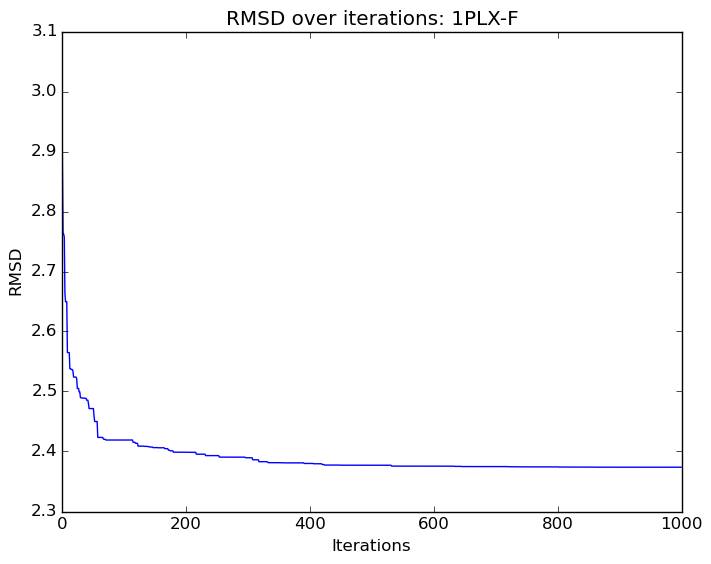
\includegraphics[width=0.7\linewidth]{1PLX-F_rmsd.png}
\end{figure}
Tempo de execução: $65$ minutos
\end{frame}

\begin{frame}
\frametitle{Resultados}
$RMSD_{C_\alpha}: 0.38657032646$

$RMSD_{backbone}: 0.827079038808$

$RMSD_{all}: 2.37386628213$ 

\begin{figure}
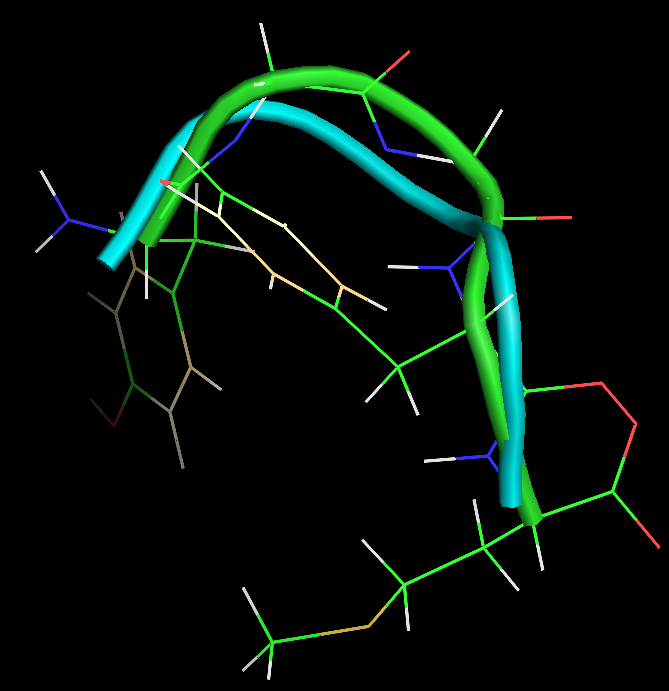
\includegraphics[width=0.5\linewidth]{1PLX-F.png}
\end{figure}
\end{frame}

\begin{frame}
\frametitle{Ângulos (1PLX x 1PLX-F)}
\begin{table}[]
\centering
\label{my-label}
\begin{tabular}{llll}
AA & PHI             &  PSI              &  OMEGA             \\
TYR         & 360.00 x 360.00 &  176.63 x -110.52 &  179.86 x -179.98  \\
GLY         & 148.48 x 124.15 &  -21.96 x    2.58 &  179.81 x -179.97  \\
GLY         & 114.02 x  84.56 &   29.89 x   27.43 &  179.75 x  179.97  \\
PHE         & -88.00 x -71.94 &  -38.16 x  -94.85 & -179.95 x  179.99  \\
MET         & -74.24 x -14.96 &  360.00 x  360.00 &  360.00 x  360.00
\end{tabular}
\end{table}
\end{frame}

%------------------------------------------------

\begin{frame}
\Huge{\centerline{Fim}}
\end{frame}

%----------------------------------------------------------------------------------------

\end{document} 